%
% exemplo genérico de uso da classe iiufrgs.cls
% $Id: iiufrgs.tex,v 1.1.1.1 2005/01/18 23:54:42 avila Exp $
%
% This is an example file and is hereby explicitly put in the
% public domain.
%
\def\crj#1{\textcolor{red}{(#1)}}
\def\todo#1{\textcolor{orange}{(#1)}}
\documentclass[cic,tc]{iiufrgs}
\usepackage{tikz}
\usepackage{tikz-3dplot}
\usetikzlibrary{calc,arrows.meta,positioning,backgrounds}
\usepackage{gensymb}
\usepackage{amsmath}
\tdplotsetmaincoords{-60}{-35}

% Para usar o modelo, deve-se informar o programa e o tipo de documento.
% Programas :
% * cic       -- Graduação em Ciência da Computação
% * ecp       -- Graduação em Ciência da Computação
% * ppgc      -- Programa de Pós Graduação em Computação
% * pgmigro   -- Programa de Pós Graduação em Microeletrônica
%
% Tipos de Documento:
% * tc                -- Trabalhos de Conclusão (apenas cic e ecp)
% * diss ou mestrado  -- Dissertações de Mestrado (ppgc e pgmicro)
% * tese ou doutorado -- Teses de Doutorado (ppgc e pgmicro)
% * ti                -- Trabalho Individual (ppgc e pgmicro)
%
% Outras Opções:
% * english    -- para textos em inglês
% * openright  -- Força início de capítulos em páginas ímpares (padrão da
% biblioteca)
% * oneside    -- Desliga frente-e-verso
% * nominatalocal -- Lê os dados da nominata do arquivo nominatalocal.def


% Use unicode
\usepackage[utf8]{inputenc}   % pacote para acentuação

% Necessário para incluir figuras
\usepackage{graphicx}         % pacote para importar figuras

\usepackage{times}            % pacote para usar fonte Adobe Times
% \usepackage{palatino}
% \usepackage{mathptmx}       % p/ usar fonte Adobe Times nas fórmulas

\usepackage[alf,abnt-emphasize=bf]{abntex2cite}	% pacote para usar citações abnt
%
% Informações gerais
%
\title{Estimativa de profundidade monocular a partir de imagens omnidirecionais}

\author{Dal'Aqua}{Lorenzo Pezzi}

% orientador e co-orientador são opcionais (não diga isso pra eles :))
\advisor[Prof.~Dr.]{Jung}{Claudio Rosito}
% \coadvisor[Prof.~Dr.]{Knuth}{Donald Ervin}

% a data deve ser a da defesa; se nao especificada, são gerados
% mes e ano correntes
\date{Janeiro}{11, 2018}

% o local de realização do trabalho pode ser especificado (ex. para TCs)
% com o comando \location:
% \location{Itaquaquecetuba}{SP}

% itens individuais da nominata podem ser redefinidos com os comandos
% abaixo:
% \renewcommand{\nominataReit}{Prof\textsuperscript{a}.~Wrana Maria Panizzi}
% \renewcommand{\nominataReitname}{Reitora}
% \renewcommand{\nominataPRE}{Prof.~Jos{\'e} Carlos Ferraz Hennemann}
% \renewcommand{\nominataPREname}{Pr{\'o}-Reitor de Ensino}
% \renewcommand{\nominataPRAPG}{Prof\textsuperscript{a}.~Joc{\'e}lia Grazia}
% \renewcommand{\nominataPRAPGname}{Pr{\'o}-Reitora Adjunta de P{\'o}s-Gradua{\c{c}}{\~a}o}
% \renewcommand{\nominataDir}{Prof.~Philippe Olivier Alexandre Navaux}
% \renewcommand{\nominataDirname}{Diretor do Instituto de Inform{\'a}tica}
% \renewcommand{\nominataCoord}{Prof.~Carlos Alberto Heuser}
% \renewcommand{\nominataCoordname}{Coordenador do PPGC}
% \renewcommand{\nominataBibchefe}{Beatriz Regina Bastos Haro}
% \renewcommand{\nominataBibchefename}{Bibliotec{\'a}ria-chefe do Instituto de Inform{\'a}tica}
% \renewcommand{\nominataChefeINA}{Prof.~Jos{\'e} Valdeni de Lima}
% \renewcommand{\nominataChefeINAname}{Chefe do \deptINA}
% \renewcommand{\nominataChefeINT}{Prof.~Leila Ribeiro}
% \renewcommand{\nominataChefeINTname}{Chefe do \deptINT}

% A seguir são apresentados comandos específicos para alguns
% tipos de documentos.

% Trabalho Individual [ti]:
% \ti{123}     % numero do TI
% \ti[II]{456} % no caso de ser o segundo TI

%
% palavras-chave
% iniciar todas com letras minúsculas, exceto no caso de abreviaturas
%
\keyword{imagens omnidirecionais}
\keyword{estimativa de profundidade}

%\settowidth{\seclen}{1.10~}

%
% inicio do documento
%
\begin{document}

% folha de rosto
% às vezes é necessário redefinir algum comando logo antes de produzir
% a folha de rosto:
% \renewcommand{\coordname}{Coordenadora do Curso}
\maketitle

% dedicatoria
% \clearpage
% \begin{flushright}
%     \mbox{}\vfill
%     {\sffamily\itshape
%       ``If I have seen farther than others,\\
%       it is because I stood on the shoulders of giants.''\\}
%     --- \textsc{Sir~Isaac Newton}
% \end{flushright}

% agradecimentos
%\chapter*{Agradecimentos}
%Agradecimentos...



% resumo na língua do documento
\begin{abstract}
    Abstract em português
\end{abstract}

% resumo na outra língua
% como parametros devem ser passados o titulo e as palavras-chave
% na outra língua, separadas por vírgulas
\begin{englishabstract}{Monocular Depth estimation on omnidirectional images}{Keywords, in, English}
    Abstract in english
\end{englishabstract}

% lista de figuras
\listoffigures

% lista de tabelas
\listoftables

% lista de abreviaturas e siglas
% o parametro deve ser a abreviatura mais longa
\begin{listofabbrv}{NCC}
	\item[CCD] \textit{Charge-coupled device}
    \item[MRF] \textit{Markov Random Field}
    \item[NCC] \textit{Normalized Cross Correlation}
\end{listofabbrv}

% % idem para a lista de símbolos
% \begin{listofsymbols}{$\alpha\beta\pi\omega$}
%     \item[$\lambda$] Longitude
%     \item[$\phi$] Latitude
% \end{listofsymbols}

% sumario
\tableofcontents

% aqui comeca o texto propriamente dito

% introducao
\chapter{Introdução}

\section{Motivação}

A estimativa de profundidade é um componente crucial para a compreensão da geometria tridimensional de uma cena. Imagens omnidirecionais, ou esféricas, possuem um campo de visão de 360\degree e oferecem informação contextual muito maior sobre a cena em relação à imagens planares comuns, logo, a estimativa de profundidade nestas imagens pode ser de utilidade para uma gama de aplicações, desde compreensão de cenas, detecção de objetos, navegação, reconstrução 3D, realidade virtual e realidade aumentada.

O método tradicional para obtenção de mapas de profundidade é o casamento estéreo, que utiliza as correspondências entre um par de imagens para estimar a profundidade em uma cena, mas requer mútliplas imagens e/ou configurações de câmeras especializadas. Há diversos resultados promissores na obtenção de mapas de profundidade a partir de uma única imagem, como os trabalhos de  \citet{Eigen2015} e \citet{Fayao2015} (Figura \ref{fig:monoDepth}), que utilizam redes neurais convolucionais. Estas redes, no entanto, são treinadas a partir de imagens planares que possuem valores de profundidades conhecidos.
\begin{figure}
    \caption{Estimativa de profundidade monocular}
    \begin{center}
        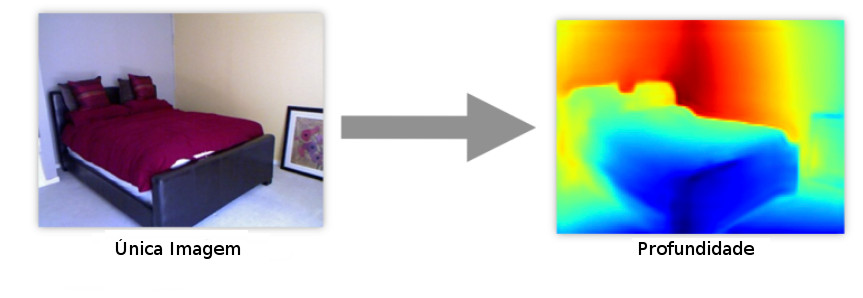
\includegraphics[width=30em]{monocular-depth.jpg}
    \end{center}
    \label{fig:monoDepth}
    \legend{Fonte: \citep{Eigen2015}, modificado}
\end{figure}
Na medida em que a utilização de câmeras omnidirecionais se popularizam em aplicações como realidade virtual e aumentada, robótica, etc. seria proveitoso utilizar estes métodos de estimativa a partir de imagens monoculares para obter mapas de profundidade a partir de uma única imagem esférica. Contudo, são escassas as bases de dados de imagens esféricas com valores de profundidades conhecidos que se assemelhem às utilizadas para o treinamento das redes com imagens planares, logo seria interessante um método que utilize as redes já treinadas para imagens planares para utilização com imagens esféricas.

\section{Objetivo}

O objetivo do trabalho é desenvolver e testar um método que utilize as técnicas de estimativa de profundidade monocular em imagens planares já existentes para obter mapas de profundidade a partir de imagens esféricas.

\section{Estrutura}

O trabalho é estruturado da seguinte forma:

\begin{itemize}
\item \textbf{Conceitos:} Apresentar os principais conceitos abordados, de modo a contextualizar a discussão posterior do desenvolvimento do método.
\item \textbf{Trabalho anterior:} Relacionar a pesquisa já realizada tanto em estimativa de profundidade quanto com imagens omnidirecionais, e contextualizar o método proposto.
\item \textbf{O método proposto:} Descrever o método desenvolvido, suas etapas e funcionamento.
\item \textbf{Resultados:} Avaliação do método e apresentação de resultados qualitativos, quantitativos e visualizações dos mapas de profundidade obtidos.
\item \textbf{Conclusão:} Discutir o desempenho do método e possibilidades de trabalho futuro.
\end{itemize}

\chapter{Conceitos}

\section{Imagens planares vs. omnidirecionais}

Uma imagem é uma representação 2D do espaço tridimensional, capturada por um meio sensível à luz, no caso de imagens digitais, sensores como CCD (\textit{Charge-coupled device}) \citep{Gonzalez}. Nesta seção detalharemos como são obtidas imagens planares, e como estas diferem das imagens omnidirecionais que são o foco deste trabalho.

\subsection{Imagens planares}

Uma câmera comum mapeia o espaço tridimensional para um plano através da projeção perspectiva. Como descrito em \citet{Szeliski}, um modelo simples para o funcionamento de uma câmera é o modelo de lentes finas. Como descrito na figura (\ref{fig:lens-fov}), o campo de visão de uma imagem obtida por uma câmera comum é o ângulo $f.o.v.$ e depende da relação entre o tamanho $W$ do sensor de imagem e da distância focal $f$ da lente. Exceto usando lentes especiais que distorcem a projeção perspectiva (e.g. \textit{fisheye}), o campo de visão será limitado em no máximo 180\degree .
\begin{figure}
    \caption{Modelo de lentes finas}
    \begin{center}
        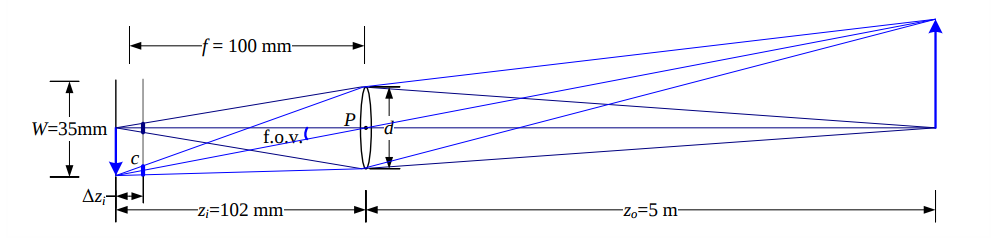
\includegraphics[width=30em]{lens-fov.png}
    \end{center}
    \label{fig:lens-fov}
    \legend{O campo de visão ($f.o.v.$) é dependente da proporção entre o tamanho do sensor $W$ e a distância focal $f$. Fonte: \citep{Szeliski}}
\end{figure}
\subsection{Imagens omnidirecionais}

Imagens omnidirecionais, também conhecidas como imagens esféricas, idealmente capturam a luz de todas as direções, e possuem um campo de visão de 360\degree. Como explicado na seção anterior, a projeção perspectiva é limitada a 180\degree, então, para mapear todos os pontos da esfera de raio unitário, com duas dimensões, é necessário utilizar outras projeções. Há uma míriade de projeções para projetar mapas \citep{sphereProjections}, por exemplo, cilíndricas, cônicas e azimutais. Ao longo do trabalho será utilizada somente a projeção equiretangular.

\subsubsection{Projeção equiretangular}

A projeção equiretangular é um caso específico da projeção cilíndrica equidistante. De acordo com \citet{equiretangularProjection}, as equações de mapeamento para latitude $\phi$ e longitude $\lambda$ na esfera para coordenadas horizontais $x$ e verticais $y$ na imagem se dão por:

$$ x = (\lambda - \lambda_0)\cos{\phi_1} $$
$$ y = (\phi - \phi_1)$$

Sendo $\phi_1$ o ângulo dos paralelos ao norte e sul do equador da esfera onde a escala da projeção é exata, na projeção equiretangular é $\phi_1 = 0$, e $\lambda_0$ o meridiano central do mapa, que no caso de imagens podemos definir como zero, a projeção equiretangular é simplesmente uma conversão direta de longitude na esfera para coordenada horizontal na imagem e latitude na esfera para coordenada vertical na imagem. No entanto, ângulos são contínuos, a latitude varia de 0 a $2\pi$ radianos e a longitude de 0 a $\pi$ radianos, e as coordenadas de pixel são discretas e sua variação depende da resolução da imagem, então, dada uma imagem com $W$ pixels na horizontal e $H$ pixels na vertical como na figura \ref{fig:sphericalIm}, temos as seguintes relações:

$$ \frac{x}{W} = \frac{\lambda}{2\pi}, \hspace{1em} e \hspace{1em}  \frac{y}{H} = \frac{\phi}{\pi}$$

E a partir destas relações, para qualquer pixel na coordenada $x,y$ na imagem projetada, obtemos a latitude $\phi$ e longitude $\lambda$ na esfera por:

$$ \lambda = \frac{2\pi x}{W}, \hspace{1em}  \phi = \frac{\pi y}{H}$$

\subsubsection{Captura de imagens omnidirecionais}

Como explicado anteriormente, câmeras comuns possuem um limite de campo de visão, e ainda não foi projetada uma câmera omnidirecional ideal, porém imagens omnidirecionais podem ser obtidas de múltiplas maneiras, utilizando uma ou mais câmeras comuns ou especializadas:
\begin{itemize}
\item É possível alterar a projeção da imagem obtida por uma única câmera através de lentes ou espelhos especiais (cônicos, esféricos, hiperbólicos, etc.). As lentes ou espelhos permitem que a câmera possa capturar toda a cena, ou pelo menos aumentam seu campo de visão. Exemplos são descritos em \citet{omniSingleCam1997} e \citet{omniSingleCam1998}.
\item Combinando informação obtida de múltiplas imagens em perspectiva, obtidas por múltiplas câmeras ou por uma câmera em movimento, e colando as imagens em uma única imagem panorâmica. Conhecido também como mosaico, há exemplos em \citet{omniMultiCam1994}, \citet{omniMultiCam1996} e \citet{omniMultiCam1997}.
\end{itemize}


\begin{figure}
    \caption{Imagem omnidirecional em projeção equiretangular}
    \begin{center}
        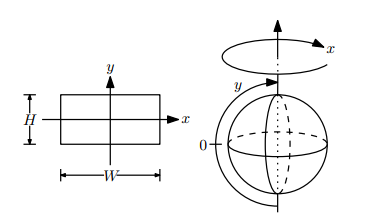
\includegraphics[width=20em]{equiretangular.png}
    \end{center}
    \label{fig:sphericalIm}
    \legend{Fonte: Jianxiong Xiao, 3D Geometry for panorama}
\end{figure}

\section{Estimativa de profundidade}

A estimativa de profundidade consiste em estimar a distância entre objetos contidos em uma ou mais imagens e uma câmera de referência. Há múltiplas aplicações em robótica, como navegação e reconhecimento de objetos, além de ser um componente essencial para a reconstrução 3D. No caso de imagens esféricas, a reconstrução 3D de uma imagem 360\degree tem aplicações diretas em realidade virtual e realidade aumentada.

O método clássico para estimativa de profundidade é o casamento estéreo, onde a profundidade é estimada utilizando a correspondência entre pixels das duas imagens. Para tanto, é preciso utilizar uma configuração de câmera cujos parâmetros sejam conhecidos. Recentemente, a aplicação de redes neurais convolucionais mostrou resultados impressionantes na estimativa de profundidade a partir de uma única imagem. No entanto, a utilização destes algoritmos com imagens 360\degree não produz a mesma qualidade de resultados, pois o treinamento destes é feito utilizando imagens perspectivas. 

A estimativa de profundidade a partir de uma única imagem é um problema desafiador, pois não se tem as indicações de profundidade da visão binocular, e não é possível se basear apenas na informação local, é necessário levar em conta o contexto global da imagem.

-sun360O método proposto neste trabalho pretende estender as técnicas de estimativa de profundidade a partir de uma única imagem em perspectiva para o domínio das imagens esféricas. Para tanto, são feitas projeções planares de seções da imagem esférica, e é estimada a profundidade de cada seção. As profundidades calculadas são projetadas de volta para o domínio esférico, porém as profundidades estimadas para cada seção não são coerentes entre si.\crj{Podes colocar uma imagem aqui para ilustrar.}
Para gerar uma mapa de profundidades suave são escolhidas seções com regiões sobrepostas, então é feita uma minimização da diferença das profundidades nas regiões sobrepostas através da ponderação da profundidade de cada seção na imagem final.


\chapter{Trabalho anterior}
\crj{Acho que podes deixar a estrutura atual, mas deixar claro que o foco é no estéreo com uma única imagem.}

\section{Estimativa de profundidade}

Esta seção cita diversos métodos para estimativa de profundidade encontrados na literatura como referência, porém o foco deste trabalho são os métodos de estimativa de profundidade monocular, ou seja, com uma única imagem.

\subsection{Múltiplas imagens}

Casamento estéreo é um problema que já foi extensivamente abordado, há múltiplas revisões da literatura, desde \citet{stereoSurvey2001}, que propuseram uma taxonomia dos algoritmos de estéreo, métricas de avaliação, e uma base de dados para teste, até mais recentemente \citet{stereoSurvey2016}, que na sua revisão avalia dezenas de algoritmos, e propõe uma taxonomia das etapas dos algoritmos de estéreo, e faz uma análise das diversas revisões da literatura já feitas.

Além do casamento de pares estéreo tradicional, mais focados na reconstrução 3D das cenas, há variações utilizando mais de duas imagens \citep{multiViewStereo2015}, ou estimando a profundidade a partir de correspondências entre imagens obtidas de uma câmera em movimento (\textit{structure from motion}) \citep{structMotion2016}. Há também métodos que estimam a profundidade sem variar a orientação da câmera, mas sim a iluminação da cena \citep{photometricStereo1989}, \citep{photometricStereo2012}, ou os parâmetros da câmera, tipicamente o foco \citep{defocus1987}, \citep{defocus2015}.

\subsection{Única imagem}

Sem as informações de profundidades fornecidas pela visão binocular, a estimativa de profundidade pode ser vista como um problema de aprendizado, como exemplificado por \citet{Saxena2005} e \citet{Saxena2008}, que abordaram o problema como um problema de aprendizado supervisionado, e através de campos aleatórios de Markov (\textit{Markov Random Fields}, ou MRF), obtiveram mapas de profundidade razoavelmente corretos.

Semantic labels: \citet{Liu2010}

Convolutional Neural networks: 
\citet{Fayao2015}, \citet{Eigen2014}, \citet{Eigen2015}, \citet{Kuznietsov2017}, \citet{Li2017}

Unsupervised: \citet{Godard2016}, \citet{Zhou2017}


\section{Imagens omnidirecionais}

\subsection{Casamento estéreo omnidirecional}
Multiview stereo omnidirecional: \citet{Li2001}

Hardware especializado para stereo omnidirecional (robotics): \citet{gluckman1998}, \citet{Koyasu2001} (+atual): \citet{Lin2014}

Single image depth with structured light: \citet{Orghidan2005}

\subsection{Outros}
Projeção da esfera para plano: \citet{sun360}

Extensão de técnicas planares para 360: \citet{flat2sphere}

3D reconstruction from spherical images: \citet{panoContext}

\chapter{O método proposto}

\section{Visão geral do método}

O método proposto neste trabalho pretende estender qualquer técnica de estimativa de profundidade de imagens planares para ser utilizada com imagens esféricas. O método consiste de múltiplas etapas sequenciais, que chamaremos de nosso \textit{pipeline}. A imagem original esférica, na projeção equiretangular passa pelas etapas de processamento descritas na Figura~\ref{fig:pipeline}.

\begin{figure}
    \caption{Etapas do \textit{pipeline}}
    \begin{center}
        \begin{picture}(450,100)
            \put(0,20){\line(0,1){50}}
            \put(0,20){\line(1,0){90}}
            \put(90,70){\line(0,-1){50}}
            \put(90,70){\line(-1,0){90}}
            \put(90,45){\vector(1,0){10}}
            \put(10,48){Seccionamento}
            \put(20,38){e projeção}
            \put(100,20){\line(0,1){50}}
            \put(100,20){\line(1,0){90}}
            \put(190,70){\line(0,-1){50}}
            \put(190,70){\line(-1,0){90}}
            \put(190,45){\vector(1,0){10}}
            \put(120,48){Estimativa}
            \put(108,38){de profundidade}
            \put(200,20){\line(0,1){50}}
            \put(200,20){\line(1,0){70}}
            \put(270,70){\line(0,-1){50}}
            \put(270,70){\line(-1,0){70}}
            \put(270,45){\vector(1,0){10}}
            \put(207,48){Reprojeção}
            \put(208,38){para esfera}
            \put(280,20){\line(0,1){50}}
            \put(280,20){\line(1,0){70}}
            \put(350,70){\line(0,-1){50}}
            \put(350,70){\line(-1,0){70}}
            \put(350,45){\vector(1,0){10}}
            \put(287,42.5){Ponderação}
            \put(360,20){\line(0,1){50}}
            \put(360,20){\line(1,0){80}}
            \put(440,70){\line(0,-1){50}}
            \put(440,70){\line(-1,0){80}}
            \put(366,42.5){Reconstrução}
        \end{picture}
    \end{center}
    \label{fig:pipeline}
    \legend{Fonte: O Autor}
\end{figure}

Inicialmente, a imagem esférica na projeção equiretangular é dividida em várias seções com sobreposição, e estas são projetadas para imagens planares. A estimativa de profundidade é realizada nestas projeções planares, e qualquer técnicas de estimativa de profundidade a partir de uma única imagem pode ser utilizada para isso.  As profundidades estimadas são projetadas de volta para o domínio esférico, formando um conjunto de imagens equiretangulares onde temos apenas uma parte da profundidade da esfera em cada uma. As técnicas utilizadas para estimativa de profundidade, no entanto, não impõem coerência entre as profundidades estimadas em cada seção da esfera, requerendo uma fusão das profundidades geradas em cada seção a fim de aprimorar a coerência global entre as estimativas de cada seção. Por fim, o método minimiza a diferença entre as profundidades de cada seção nas regiões de sobreposição. Como ainda há casos onde a diferença pode ser consideravelmente diferente de zero, é feito um \textit{blending} entre as profundidades estimadas para cada seção a fim de gerar um mapa de profundidades suave. Cada etapa será descrita em detalhes nas seções a seguir.

\section{Seccionamento e projeção para o plano}

Esfera seccionada em $N$ planos, com sobreposição porque precisamos de informação redundante para gerar a coerência global. Cada plano com FOV de $\theta$, e $\theta/2$ de diferença entre as seções, logo há 45\degree de overlap.

A projeção é calculada utilizando a distância focal conhecida $2\pi W$ (Figura \ref{fig:sphericalIm})

Pega tamanho de imagem destino e ângulos de projeção phi, theta

calcula para cada pixel os ângulos phii thetai do pixel

divide os ângulos pela distancia focal 2piw ou pi*H para encontrar os pixels da imagem esférica que correspondem.

interpola a imagem esférica porque os pixels não são inteiros.



\section{Estimativa de profundidade}

O método é independente da técnica de estimativa de profundidade utilizada, só é necessário que seja uma técnica de estimativa a partir de uma única imagem. Os resultados com redes neurais são impressionantes, escolhemos a rede do Fayao por ter código disponível. Utilizamos as redes como um \textit{blackbox}.

Código usado foi de \citet{Fayao2015}.

\section{Projetando a seção de volta para a esfera}

Pega todos os ângulos que tem na imagem planar (precisa do FOV)

Converte os ângulos pros index dos pixels.

faz o validmap com os pixels da esfera que pertencem à seção.

interpola a imagem planar pra formar a seção esférica

\section{Ponderação dos mapas de profundidade de cada seção}

Temos várias seções esféricas com overlap, sabemos que nos overlaps queremos que os valores sejam iguais. Para cada overlap, geramos pesos linha a linha para ponderar os valores de profundidade. 

Minimizar diferença entre profundidades estimadas:

Sejam $I(x,y)$ uma imagem esférica, $D_L(x,y)$ e $D_R(x,y)$ estimativas de profundidade de duas seções de $I$, $P$ o conjunto dos pixels e $L$ o conjunto das linhas da região de sobreposição entre estas duas seções de $I$, queremos calcular pesos $w_{kL}$ e $w_{kR}$ para cada linha $k$, tal que $ k \in L$ para ponderar as linhas destas seções de $I$. Para isso, queremos escolher pesos que
$$ W_D = \sum_{(i,j) \in P}(w_{iL}D_L(i,j)-w_{iR}D_R(i,j)) $$
$$ W_C = \sum_{(i,j) \in P}T(i,j)((w_{iL}-w_{i+1L})+(w_{iR}-w_{i+1R}))$$
$$T(i,j) = \begin{cases}
  \alpha, $ se $ |I(i,j)-I(i+1,j)| < \gamma \\
  \beta, $ se $  |I(i,j)-I(i+1,j)| \geq \gamma  \\
\end{cases}$$

(Equação do sistema). A solução do sistema se dá por SVD (citar?), mas podemos variar as ponderações das equações entre pesos ou entre profundidades.

Cada seção da esfera tem duas regiões de overlap, que geram pesos diferentes em cada parte da imagem. É feita uma interpolação destes pesos à medida que se encontra a metade da seção esférica. Cada seção gera tem então mapas de disparidades mais coerentes entre si.

\section{Reconstrução do mapa de profundidade completo}

Ainda há diferença entre os mapas, então região de overlap tem que ser blended. Fizemos um alpha blending simples baseado na proximidade do pixel de cada projeção, para gerar um mapa de profundidade suave. Gera alguns artefatos na borda das regiões de overlap, onde não tem blending.

\chapter{Resultados}
\section{Dataset}
\todo{Vistas sintéticas com o ground truth, perguntar p/ Thiago os detalhes da cena}
\todo{Pegar um dataset do SUN360 para visualizar somente}

\section{Visualização}

\todo{Colocar alguns mapas gerados, talvez vistas da point cloud?}

\section{Métricas}

A métrica para avaliação do método escolhida foi a Correlação Cruzada Normalizada (\textit{Normalized Cross-Correlation}, ou NCC) \citep{NCC2006}. A $NCC$ entre duas imagens de profundidade, $f$ e $g$, onde $n$ é o número de pixels das imagens $\sigma_i$ é o desvio padrão da imagem $i$ e $\bar{i}$ é a média dos valores da imagem $i$, é descrita pela fórmula a seguir:

$$NCC(f,g) = \frac{1}{n \sigma_f \sigma_g}\sum_{x=0}^{n}(f(x)-\bar{f})(g(x)-\bar{g})$$

A métrica varia entre $[-1,1]$, sendo -1 a diferença máxima entre as imagens e 1 a diferença mínima.

\begin{table}[h]
    \caption{Tabela com métricas dos resultados FOV 90\degree}
    \vspace{0.5em}
    \centering
        \begin{tabular}{|c|c|c|c|}
          \hline
          \textit{Imagem} & \textit{NCC seções} & \textit{NCC CNN} & \textit{Diferença} \\
          \hline
          \hline
          classroom000 & -0.25830 & -0.28226 & 0.02395 \\
          classroom001 & 0.41962 & -0.12315 & 0.54277 \\
          classroom002 & 0.28472 & -0.21357 & 0.49829 \\
          classroom003 & 0.37980 & -0.18954 & 0.56934 \\
          classroom004 & 0.13828 & -0.27350 & 0.41178 \\
          classroom005 & 0.26561 & -0.22434 & 0.48995 \\
          classroom006 & 0.17824 & -0.06920 & 0.24744 \\
          classroom007 & 0.44273 & -0.18177 & 0.62450 \\
          classroom008 & 0.23351 & -0.22762 & 0.46114 \\
          classroom009 & 0.39315 & -0.06912 & 0.46228 \\
          classroom010 & 0.30436 & -0.11798 & 0.42234 \\
          classroom011 & -0.10358 & -0.22381 & 0.12024 \\
          classroom012 & 0.39815 & -0.20630 & 0.60445 \\
          classroom013 & 0.00997 & -0.18586 & 0.19582 \\
          classroom014 & 0.20669 & -0.28898 & 0.49567 \\
          classroom075 & 0.28160 & -0.28071 & 0.56231 \\
          classroom085 & 0.26957 & -0.28733 & 0.55690 \\
          classroom095 & 0.35448 & -0.26133 & 0.61581 \\
          classroom105 & 0.35337 & -0.25931 & 0.61268 \\
          classroom115 & 0.34220 & -0.26143 & 0.60363 \\
          classroom125 & 0.35067 & -0.26573 & 0.61640 \\
          classroom135 & 0.36270 & -0.25510 & 0.61780 \\
          classroom145 & 0.31987 & -0.28003 & 0.59990 \\
          classroom150 & 0.30897 & -0.24498 & 0.55395 \\
          classroom155 & 0.32294 & -0.25103 & 0.57397 \\
          classroom165 & 0.35006 & -0.24283 & 0.59290 \\
          classroom175 & 0.33943 & -0.23062 & 0.57005 \\
          classroom185 & 0.33393 & -0.24386 & 0.57779 \\
          classroom195 & 0.32183 & -0.25503 & 0.57685 \\
          \hline
          \hline
          mean & 0.27257 & -0.22401 & 0.49658 \\
          \hline
        \end{tabular}
    \vspace{0.5em}
    \legend{Fonte: O Autor}
    \label{tbl:results1}
\end{table}

\begin{table}[h]
    \caption{Tabela com métricas dos resultados FOV 120\degree}
    \vspace{0.5em}
    \centering
        \begin{tabular}{|c|c|c|c|}
          \hline
          \textit{Imagem} & \textit{NCC seções} & \textit{NCC CNN} & \textit{Diferença} \\
          \hline
          \hline
          classroom000 & -0.17032 & -0.21705 & 0.04673 \\
          classroom001 & 0.42219 & -0.10831 & 0.53051 \\
          classroom002 & 0.31102 & -0.20685 & 0.51787 \\
          classroom003 & 0.35680 & -0.15697 & 0.51377 \\
          classroom004 & 0.20508 & -0.23831 & 0.44338 \\
          classroom005 & 0.34369 & -0.18891 & 0.53260 \\
          classroom006 & 0.19693 & -0.05349 & 0.25042 \\
          classroom007 & 0.47997 & -0.15913 & 0.63910 \\
          classroom008 & 0.27671 & -0.22065 & 0.49736 \\
          classroom009 & 0.44129 & -0.05070 & 0.49200 \\
          classroom010 & 0.33796 & -0.10223 & 0.44019 \\
          classroom011 & -0.01260 & -0.19751 & 0.18491 \\
          classroom012 & 0.41223 & -0.18498 & 0.59721 \\
          classroom013 & 0.12704 & -0.14514 & 0.27218 \\
          classroom014 & 0.30762 & -0.25593 & 0.56355 \\
          classroom075 & 0.32709 & -0.23729 & 0.56438 \\
          classroom085 & 0.32512 & -0.24758 & 0.57270 \\
          classroom095 & 0.31677 & -0.22659 & 0.54336 \\
          classroom105 & 0.33640 & -0.21739 & 0.55379 \\
          classroom115 & 0.34648 & -0.22978 & 0.57626 \\
          classroom125 & 0.36710 & -0.23235 & 0.59945 \\
          classroom135 & 0.36841 & -0.22080 & 0.58921 \\
          classroom145 & 0.35844 & -0.24526 & 0.60370 \\
          classroom150 & 0.33417 & -0.21547 & 0.54964 \\
          classroom155 & 0.33783 & -0.22376 & 0.56159 \\
          classroom165 & 0.37149 & -0.21825 & 0.58974 \\
          classroom175 & 0.37054 & -0.20718 & 0.57773 \\
          classroom185 & 0.37027 & -0.21435 & 0.58462 \\
          classroom195 & 0.39620 & -0.23381 & 0.63001 \\
          \hline
          \hline
		  mean & 0.30903 & -0.19504 & 0.50407 \\
          \hline
        \end{tabular}
    \vspace{0.5em}
    \legend{Fonte: O Autor}
    \label{tbl:results1}
\end{table}


\chapter{Conclusões}

\section{Trabalho futuro}
Foi feita uma segunda formulação com um peso por pixel, mas a complexidade polinomial da solução por SVD tornou a solução imprática para imagens de tamanho real. É possível fazer um \textit{downscaling} e ter um peso a cada x pixels, mas ainda assim fica com muitos artefatos...\crj{Acho que podes deixar isso como future work.}

\bibliographystyle{abntex2-alf}
\bibliography{biblio}

\end{document}